\documentclass[12pt,a4paper]{article}
\usepackage[utf8]{inputenc}
\usepackage[margin=1in]{geometry}
\usepackage{graphicx}
\usepackage{xcolor}
\usepackage{tikz}
\usepackage{tcolorbox}
\usepackage{enumitem}
\usepackage{multicol}
\usepackage{hyperref}
\usepackage{fontawesome5}
\usepackage{amsmath}

\usetikzlibrary{shapes.geometric, arrows, positioning, shadows}

% Define colors
\definecolor{primaryblue}{RGB}{79, 70, 229}
\definecolor{secondarypurple}{RGB}{147, 51, 234}
\definecolor{successgreen}{RGB}{34, 197, 94}
\definecolor{warningorange}{RGB}{251, 146, 60}
\definecolor{lightgray}{RGB}{243, 244, 246}

% Custom boxes
\newtcolorbox{keypoint}{
  colback=primaryblue!5,
  colframe=primaryblue,
  fonttitle=\bfseries,
  title=Key Point,
  left=5pt,
  right=5pt
}

\newtcolorbox{example}{
  colback=successgreen!5,
  colframe=successgreen,
  fonttitle=\bfseries,
  title=Example,
  left=5pt,
  right=5pt
}

\newtcolorbox{warning}{
  colback=warningorange!5,
  colframe=warningorange,
  fonttitle=\bfseries,
  title=Important to Know,
  left=5pt,
  right=5pt
}

\title{\textbf{\Huge SwitchIT Career Companion AI}\\[0.5cm]
\Large A Simple Guide to Our Smart Career Assistant\\[0.3cm]
\large Understanding the Technology Behind Your Personal Career Mentor}

\author{SwitchIT Development Team}
\date{\today}

\begin{document}

\maketitle

\begin{abstract}
This document explains in simple terms how we're building an intelligent AI assistant for SwitchIT that will help users with their careers. Think of it as having a friendly career mentor available 24/7 who learns about the job market, remembers your journey, and provides personalized guidance. We'll walk through what it does, how it works, and why it's designed this way — all without requiring any technical knowledge.
\end{abstract}

\newpage
\tableofcontents
\newpage

%===============================================
\section{What Are We Building?}
%===============================================

\subsection{The Big Picture}

Imagine having a personal career coach who:

\begin{itemize}[leftmargin=*]
  \item \textbf{Chats with you naturally} — Like texting a friend, not filling out forms
  \item \textbf{Remembers everything} — Recalls your goals, interviews, and conversations from months ago
  \item \textbf{Asks smart questions} — Learns about your experiences to help you and others
  \item \textbf{Provides insights} — Tells you what others experienced at companies you're interested in
  \item \textbf{Supports you daily} — Celebrates wins, helps with setbacks, guides your growth
\end{itemize}

\begin{keypoint}
\textbf{Main Goal:} Transform SwitchIT from a professional profile platform into a dynamic career growth platform with an AI companion that actively helps you succeed.
\end{keypoint}

\subsection{What Makes This Different?}

Unlike LinkedIn or other platforms, our AI companion is:

\begin{enumerate}[leftmargin=*]
  \item \textbf{Proactive} — It asks you questions to understand and help you better
  \item \textbf{Learning constantly} — It gathers insights about the job market from all users
  \item \textbf{Cost-effective} — Designed to be affordable to run, so it's sustainable long-term
  \item \textbf{Privacy-focused} — Your data is yours, with clear controls over what's shared
\end{enumerate}

\begin{example}
\textbf{Real-world scenario:}

Sarah tells the AI companion she has an interview at Google next week. The AI:
\begin{itemize}
  \item Remembers this and asks about it after the interview
  \item Shares anonymized insights from others who interviewed at Google
  \item Tracks her progress toward her goal of "landing a software engineer role"
  \item Later, Sarah's experience (anonymized) helps other users preparing for Google interviews
\end{itemize}
\end{example}

%===============================================
\section{The Three Core Capabilities}
%===============================================

\subsection{Capability 1: Market Intelligence Gathering}

\textbf{What it means:} The AI collects valuable information about jobs, companies, and the market.

\textbf{How it works:}
\begin{itemize}
  \item When you chat about your job search, the AI identifies useful insights
  \item For example, if you mention "I got offered \$95,000 for a frontend developer role in Austin," the AI notes this
  \item Over time, it builds a database of salary ranges, interview experiences, and company cultures
\end{itemize}

\textbf{Why it matters:}
\begin{itemize}
  \item You get insights like "Based on 127 experiences, Google's interview process takes 4-6 weeks"
  \item The platform becomes smarter and more valuable as more people use i
  \item Everyone benefits from collective knowledge while maintaining privacy
\end{itemize}

\begin{figure}[h]
\centering
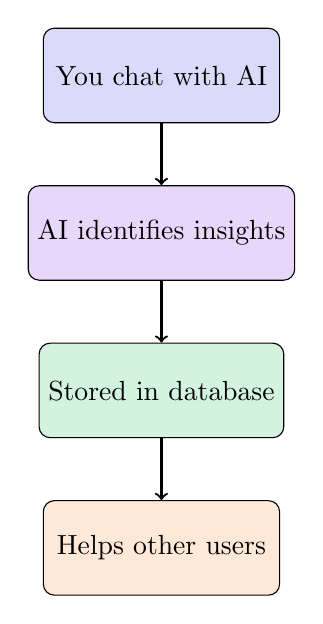
\begin{tikzpicture}[node distance=2cm]
  % Nodes
  \node[draw, rectangle, rounded corners, fill=primaryblue!20, minimum width=3cm, minimum height=1.2cm] (user) {You chat with AI};
  \node[draw, rectangle, rounded corners, fill=secondarypurple!20, minimum width=3cm, minimum height=1.2cm, below of=user] (extract) {AI identifies insights};
  \node[draw, rectangle, rounded corners, fill=successgreen!20, minimum width=3cm, minimum height=1.2cm, below of=extract] (store) {Stored in database};
  \node[draw, rectangle, rounded corners, fill=warningorange!20, minimum width=3cm, minimum height=1.2cm, below of=store] (help) {Helps other users};

  % Arrows
  \draw[->, thick] (user) -- (extract);
  \draw[->, thick] (extract) -- (store);
  \draw[->, thick] (store) -- (help);
\end{tikzpicture}
\caption{How intelligence flows through the system}
\end{figure}

\subsection{Capability 2: Conversational Memory}

\textbf{What it means:} The AI remembers your previous conversations and context.

\textbf{How it works:}
\begin{itemize}
  \item Every message is stored in a database
  \item When you chat, the AI reviews recent conversations to maintain contex
  \item It uses advanced techniques to find relevant past discussions (even from months ago)
\end{itemize}

\begin{example}
\textbf{Week 1:} You tell the AI "I'm learning React for frontend development."

\textbf{Week 4:} You say "I just finished my portfolio."

\textbf{AI Response:} "That's awesome! How did your React learning go? Can I see your portfolio to provide feedback?"
\end{example}

\subsection{Capability 3: Adaptive Questioning}

\textbf{What it means:} The AI asks the right questions at the right time to gather insights.

\textbf{How it works:}
\begin{itemize}
  \item The AI has a question bank (e.g., "How's your job search going?", "What's the interview process like?")
  \item It selects questions based on:
    \begin{itemize}
      \item Your career stage (student, early career, senior, etc.)
      \item How long since it last asked a question (avoids being annoying)
      \item Your engagement level (if you give short answers, it asks less)
      \item The conversation contex
    \end{itemize}
  \item Questions appear naturally in conversation, not like a survey
\end{itemize}

\begin{warning}
The AI will \textbf{never bombard you} with questions. It's designed to:
\begin{itemize}
  \item Ask at most 1 probing question per day
  \item Only ask when you seem engaged
  \item Make questions feel natural and conversational
  \item Let you skip questions you don't want to answer
\end{itemize}
\end{warning}

%===============================================
\section{How We're Keeping Costs Low}
%===============================================

\subsection{Why Cost Matters}

Running an AI system can be expensive because:
\begin{itemize}
  \item Every time the AI responds, we pay a third-party service (like OpenAI)
  \item Storing large amounts of data costs money
  \item Processing and searching through conversations requires computing power
\end{itemize}

Our goal is to keep monthly costs around \textbf{\$20-40 for 1,000 active users}, which is 95\% cheaper than typical AI systems.

\subsection{Five Cost-Saving Strategies}

\begin{enumerate}
  \item \textbf{Use a Cheaper AI Model}

  \begin{itemize}
    \item Instead of GPT-4 (very expensive), we use GPT-3.5-turbo (much cheaper)
    \item GPT-3.5 is still very capable for conversations and costs 95\% less
    \item Cost: \$0.0015 per 1,000 words vs \$0.03 per 1,000 words
  \end{itemize}

  \item \textbf{Smart Caching}

  \begin{itemize}
    \item If multiple users ask similar questions, we reuse the AI's previous answer
    \item Example: "What should I wear to an interview?" likely has the same answer for everyone
    \item This can reduce API calls by 30-50\%
  \end{itemize}

  \item \textbf{Keep Responses Concise}

  \begin{itemize}
    \item The AI is instructed to give helpful but brief responses (2-3 sentences)
    \item Shorter responses = fewer words = lower cos
    \item Users get answers faster, and we save money
  \end{itemize}

  \item \textbf{Free Data Storage}

  \begin{itemize}
    \item We use PostgreSQL (our existing database) instead of expensive specialized services
    \item We add a free extension called "pgvector" for smart search capabilities
    \item This saves \$70/month compared to paid alternatives
  \end{itemize}

  \item \textbf{Conversation History Limits}

  \begin{itemize}
    \item The AI only reviews the 10-15 most recent messages per conversation
    \item Earlier messages are stored but not sent to the AI each time (to reduce costs)
    \item For older context, we use smart search to find only relevant past conversations
  \end{itemize}
\end{enumerate}

\subsection{Cost Breakdown}

\begin{table}[h]
\centering
\begin{tabular}{|l|r|l|}
\hline
\textbf{Expense} & \textbf{Monthly Cost} & \textbf{Notes} \\
\hline
OpenAI API (GPT-3.5) & \$20-40 & Based on 1,000 users, 20 messages each \\
Database Storage & \$0 & Using existing PostgreSQL \\
Vector Search & \$0 & Free pgvector extension \\
Caching System & \$0 & Self-hosted Redis (free tier) \\
\hline
\textbf{TOTAL} & \textbf{\$20-40} & \textbf{About \$0.02-0.04 per user} \\
\hline
\end{tabular}
\caption{Monthly operational costs for 1,000 active users}
\end{table}

\begin{keypoint}
\textbf{For comparison:} The original plan with GPT-4 and paid services would cost \$500-2,000/month. Our optimized approach saves over 95\% while maintaining excellent quality.
\end{keypoint}

%===============================================
\section{The Implementation Journey (Step-by-Step)}
%===============================================

\subsection{Overview: Backend First, Then Frontend}

We're building this in two main phases:
\begin{enumerate}
  \item \textbf{Phase 1: Backend (the "engine")} — Build the brain and data systems
  \item \textbf{Phase 2: Frontend (the "interface")} — Create the chat window users see
\end{enumerate}

\textbf{Why backend first?}
\begin{itemize}
  \item The "brain" needs to work before we build the "face"
  \item We can test the AI's responses without needing a fancy interface
  \item Backend is more complex and has more risks, so we tackle it firs
\end{itemize}

\subsection{Phase 1: Building the Backend}

Think of the backend as the invisible machinery that makes everything work.

\subsubsection{Database Setup }

\textbf{What we're doing:} Creating organized storage spaces for all the data.

\textbf{In simple terms:}
\begin{itemize}
  \item Like creating filing cabinets with labeled drawers
  \item One drawer for conversations, another for user profiles, another for insights, etc.
  \item We create 6 different "tables" (organized storage spaces)
\end{itemize}

\textbf{Tables we create:}
\begin{enumerate}
  \item \texttt{companion\_conversations} — Every message sent/received
  \item \texttt{companion\_user\_profiles} — Your preferences and career info
  \item \texttt{market\_insights} — Collected job market intelligence
  \item \texttt{probing\_questions} — Question bank for the AI to choose from
  \item \texttt{user\_question\_history} — Which questions we've asked you
  \item \texttt{conversation\_cache} — Saved responses to save money
\end{enumerate}

\textbf{Success marker:} All 6 storage spaces exist and are ready to use.

\subsubsection{Installing Dependencies }

\textbf{What we're doing:} Getting the tools and services we need.

\textbf{In simple terms:}
\begin{itemize}
  \item Like buying ingredients before cooking
  \item We install software packages that help us:
    \begin{itemize}
      \item Talk to OpenAI (the AI provider)
      \item Search through conversations efficiently
      \item Cache responses to save money
      \item Count words/tokens for cost tracking
    \end{itemize}
\end{itemize}

\textbf{Success marker:} All tools are installed without errors.

\subsubsection{Building Core Services }

\textbf{What we're doing:} Creating the fundamental building blocks.

\textbf{The four services:}

\begin{enumerate}
  \item \textbf{Cache Service }

  \textit{Purpose:} Remember and reuse previous AI responses.

  \textit{How it works:} If someone asks "How do I prepare for interviews?" and we've answered this before, we retrieve the saved answer instead of asking OpenAI again (saves money).

  \item \textbf{LLM Service }

  \textit{Purpose:} Communicate with OpenAI's AI system.

  \textit{How it works:} This is the "translator" that sends your message to OpenAI and brings back the AI's response. It also:
  \begin{itemize}
    \item Checks the cache first (to save money)
    \item Keeps track of how many words we're sending (cost control)
    \item Makes sure responses are concise
  \end{itemize}

  \item \textbf{Vector Service }

  \textit{Purpose:} Find relevant past conversations.

  \textit{How it works:} Converts conversations into numerical "fingerprints" that can be compared. When you ask about "Google interviews," it can find all past conversations about Google, even if they didn't use those exact words.

  \textit{Analogy:} Like a smart librarian who understands topics, not just searches for exact word matches.

  \item \textbf{Context Builder }

  \textit{Purpose:} Assemble all relevant information before the AI responds.

  \textit{How it works:} Before generating a response, it gathers:
  \begin{itemize}
    \item Your last 10-15 messages
    \item Your profile (career stage, goals, etc.)
    \item Your recent SwitchIT activity (posts, connections)
    \item Relevant past conversations (found using Vector Service)
  \end{itemize}

  All this gives the AI context to provide personalized, informed responses.
\end{enumerate}

\textbf{Success marker:} Each service has tests that prove it works correctly.

\subsubsection{Intelligence Layer }

\textbf{What we're doing:} Teaching the AI to extract and use market insights.

\begin{enumerate}
  \item \textbf{Intelligence Service }

  \textit{Purpose:} Identify valuable information in conversations.

  \textit{Example:} When you say "I interviewed at Microsoft and they asked me 3 coding questions about data structures," the AI recognizes this as valuable insight and saves it as:
  \begin{itemize}
    \item Type: Interview Experience
    \item Company: Microsof
    \item Details: Coding questions, data structures focus
  \end{itemize}

  \item \textbf{Probing Service }

  \textit{Purpose:} Decide when and what to ask.

  \textit{How it works:}
  \begin{itemize}
    \item Checks: When did we last ask a question? (wait at least 24 hours)
    \item Checks: Is the user engaged? (if giving short answers, don't ask)
    \item Checks: What stage is the user at? (students get different questions than seniors)
    \item Selects the most relevant question from the question bank
  \end{itemize}

  \item \textbf{Question Bank Setup }

  \textit{Purpose:} Create the initial set of questions.

  \textit{Examples of questions in the bank:}
  \begin{itemize}
    \item "What stage are you at in your career journey?"
    \item "Have you had any interviews recently? How did they go?"
    \item "What salary range are companies offering you?"
    \item "How would you describe your workplace culture?"
  \end{itemize}
\end{enumerate}

\textbf{Success marker:} The AI can extract insights from test messages and select appropriate questions.

\subsubsection{Conversation Engine }

\textbf{What we're doing:} Building the "brain" that orchestrates everything.

\textbf{What the Conversation Engine does:}
\begin{enumerate}
  \item Receives your message
  \item Saves it to the database
  \item Gathers context (using Context Builder)
  \item Sends context + message to OpenAI (using LLM Service)
  \item Receives AI response
  \item Extracts insights from your message (using Intelligence Service, runs in background)
  \item Decides if it should ask a probing question (using Probing Service)
  \item Combines AI response + optional question
  \item Saves and returns the complete response
\end{enumerate}

\textbf{Success marker:} A complete conversation flow works from start to finish.

\subsubsection{API Endpoints }

\textbf{What we're doing:} Creating the "doors" that let the frontend communicate with the backend.

\textbf{In simple terms:}
\begin{itemize}
  \item Like creating phone numbers that the website can call to request services
  \item Each endpoint is a specific function (send message, get history, check onboarding, etc.)
\end{itemize}

\textbf{Endpoints we create:}
\begin{itemize}
  \item \texttt{POST /api/v1/companion/chat} — Send a message, get AI response
  \item \texttt{GET /api/v1/companion/conversations} — Retrieve message history
  \item \texttt{GET /api/v1/companion/onboarding/status} — Check if user needs onboarding
  \item \texttt{POST /api/v1/companion/onboarding/complete} — Mark onboarding done
\end{itemize}

\textbf{Success marker:} All endpoints respond correctly when tested with tools like Postman.

\subsubsection{Testing \& Integration }

\textbf{What we're doing:} Making sure everything works together and meets our goals.

\begin{enumerate}
  \item \textbf{Integration Testing }

  \textit{Test:} Does the companion work with the existing SwitchIT platform?

  \textit{Checks:}
  \begin{itemize}
    \item Can users log in with their SwitchIT account?
    \item Does the AI see their SwitchIT profile and activity?
    \item Do all the services work together smoothly?
  \end{itemize}

  \item \textbf{Load Testing }

  \textit{Test:} Can it handle many users at once?

  \textit{Checks:}
  \begin{itemize}
    \item Simulate 100+ users chatting simultaneously
    \item Measure response time (goal: under 2 seconds)
    \item Check if any errors occur under load
  \end{itemize}

  \item \textbf{Cost Analysis }

  \textit{Test:} Are we staying within budget?

  \textit{Checks:}
  \begin{itemize}
    \item Track actual API costs for test conversations
    \item Verify caching is working (reducing costs)
    \item Confirm cost per conversation is under \$0.03
  \end{itemize}
\end{enumerate}

\textbf{Success markers:}
\begin{itemize}
  \item Response time < 2 seconds
  \item Cost per conversation < \$0.03
  \item No critical errors during load testing
\end{itemize}

\subsection{Phase 2: Building the Frontend}

The frontend is what users actually see and interact with.

\subsubsection{Create Chat Interface }

\textbf{What we're doing:} Building the chat window that appears on SwitchIT.

\textbf{Visual components:}
\begin{itemize}
  \item \textbf{Floating button} — A purple button in the bottom-right corner
  \item \textbf{Chat window} — Pops up when you click the button (like Intercom or customer support chats)
  \item \textbf{Message bubbles} — Your messages in blue, AI messages in white
  \item \textbf{Typing indicator} — Shows when AI is "thinking"
  \item \textbf{Minimize/maximize buttons} — So you can keep it open while browsing
\end{itemize}

\textbf{Features implemented:}
\begin{enumerate}
  \item Basic chat layou
  \item Message rendering with timestamps
  \item Onboarding flow (shows welcome message for new users)
  \item Animations and polish (smooth transitions, hover effects)
\end{enumerate}

\textbf{Success marker:} Chat interface looks professional and works smoothly (tested with fake responses first).

\subsubsection{Connect to Backend}

\textbf{What we're doing:} Linking the chat interface to the real AI backend.

\textbf{First: } Create the communication layer (API service)
\begin{itemize}
  \item Code that sends messages to backend endpoints
  \item Code that receives and displays AI responses
  \item Error handling (what happens if the connection fails)
\end{itemize}

\textbf{Then:} Test with real backend
\begin{itemize}
  \item Send actual messages to the AI
  \item Verify responses appear correctly
  \item Check that conversation history loads properly
\end{itemize}

\textbf{Success marker:} Can have a real conversation with the AI through the interface.

\subsubsection{Integrate with SwitchIT}

\textbf{What we're doing:} Embedding the companion into the main SwitchIT platform.

\textbf{First:} Add floating button to SwitchIT pages
\begin{itemize}
  \item Button appears on every page after login
  \item Clicking opens the chat window
  \item Window stays open when navigating between pages
\end{itemize}

\textbf{Then:} Full user flow testing
\begin{itemize}
  \item Log in to SwitchIT
  \item Click profile, browse jobs, etc.
  \item Open companion cha
  \item Have conversation while using other features
  \item Verify everything works seamlessly
\end{itemize}

\textbf{Success marker:} Companion feels like a natural part of SwitchIT, not a separate tool.

\subsubsection{Onboarding Polish}

\textbf{What we're doing:} Perfect the new user experience.

\textbf{Features:}
\begin{itemize}
  \item \textbf{First-time users} see a notification badge on the companion button
  \item \textbf{Welcome message} introduces the AI and asks initial questions
  \item \textbf{Progress tracking} shows how much of onboarding is complete
  \item \textbf{Returning users} skip onboarding and jump straight to cha
\end{itemize}

\textbf{Onboarding questions (asked conversationally):}
\begin{enumerate}
  \item What stage are you at in your career?
  \item Are you currently job searching?
  \item What roles are you interested in?
  \item Can I help track your career goals?
\end{enumerate}

\textbf{Success marker:} Smooth onboarding experience that doesn't feel like a survey.

\subsubsection{Final Testing \& Launch Prep}

\textbf{What we're doing:} Final checks before releasing to users.

\textbf{First:} Create test scenarios
\begin{itemize}
  \item New user journey (from signup to first conversation)
  \item Returning user journey (continuing previous conversation)
  \item Error scenarios (what if internet disconnects? what if AI is slow?)
\end{itemize}

\textbf{Second:} Cross-browser and mobile testing
\begin{itemize}
  \item Test on Chrome, Firefox, Safari
  \item Test on phones and tablets
  \item Fix any visual or functional issues
\end{itemize}

\textbf{Finally:} Beta launch preparation
\begin{itemize}
  \item Set up monitoring (track errors and performance)
  \item Set up cost alerts (notify if daily spending exceeds \$5)
  \item Prepare user documentation (how to use the companion)
  \item Select beta testers (10-20 users to try it first)
\end{itemize}

\textbf{Success marker:} System is stable, tested, and ready for real users.

%===============================================
\section{Privacy \& Data Protection}
%===============================================

\subsection{What Data We Collect}

\begin{enumerate}
  \item \textbf{Conversation Messages}
  \begin{itemize}
    \item Everything you type in the cha
    \item Every AI response
    \item Timestamps and conversation contex
  \end{itemize}

  \item \textbf{Career Information}
  \begin{itemize}
    \item Career stage (student, professional, etc.)
    \item Job search status
    \item Target roles and industries
    \item Goals you share
  \end{itemize}

  \item \textbf{Market Insights}
  \begin{itemize}
    \item Company names you mention
    \item Interview experiences
    \item Salary information
    \item Workplace culture feedback
  \end{itemize}

  \item \textbf{SwitchIT Activity} (what you already share on the platform)
  \begin{itemize}
    \item Your profile information
    \item Posts you create
    \item Connections you make
  \end{itemize}
\end{enumerate}

\subsection{How We Protect Your Privacy}

\begin{enumerate}
  \item \textbf{Your Data is Yours}
  \begin{itemize}
    \item You can download all your companion data anytime (as a JSON file)
    \item You can delete specific conversations or all companion data
    \item Deleted data is kept for 30 days (in case you change your mind), then permanently removed
  \end{itemize}

  \item \textbf{Data Sharing is Optional}
  \begin{itemize}
    \item By default, your insights are \textbf{private} (only you and the AI see them)
    \item You can opt-in to share anonymized insights to help other users
    \item Even if you opt-in, your name is never attached to shared data
  \end{itemize}

  \item \textbf{Anonymization}
  \begin{itemize}
    \item When insights are aggregated, all identifying information is removed
    \item Example: Instead of "Sarah said Google pays \$95K," it becomes "1 user reported Google offers in the \$90-100K range"
  \end{itemize}

  \item \textbf{Security Measures}
  \begin{itemize}
    \item All data is encrypted in storage
    \item Communication with OpenAI is encrypted
    \item Only you can access your conversations (not even other SwitchIT users)
    \item Regular security audits
  \end{itemize}

  \item \textbf{Third-Party Data}
  \begin{itemize}
    \item We send conversations to OpenAI for AI processing
    \item OpenAI's policy: They don't use your data to train their models (as of their API enterprise agreement)
    \item No data is sold to third parties
  \end{itemize}
\end{enumerate}

\begin{warning}
\textbf{Before Launch:} We need to:
\begin{itemize}
  \item Update SwitchIT's privacy policy to reflect companion data collection
  \item Get legal review for GDPR compliance (if operating in Europe)
  \item Create clear opt-in consent flow for data sharing
  \item Define data retention policy (how long we keep conversations)
\end{itemize}
\end{warning}

%===============================================
\section{How We Measure Success}
%===============================================

\subsection{Technical Success Metrics}

These measure if the system is working well technically:

\begin{table}[h]
\centering
\begin{tabular}{|l|l|l|}
\hline
\textbf{Metric} & \textbf{Target} & \textbf{What it Means} \\
\hline
Response Time & < 2 seconds & How fast AI responds \\
Uptime & 99.5\% & System availability \\
Cache Hit Rate & > 50\% & How often we reuse responses \\
Error Rate & < 1\% & How often things break \\
Cost per Conversation & < \$0.03 & Spending per chat session \\
\hline
\end{tabular}
\caption{Technical performance targets}
\end{table}

\subsection{User Success Metrics}

These measure if users find it valuable:

\begin{table}[h]
\centering
\begin{tabular}{|l|l|l|}
\hline
\textbf{Metric} & \textbf{Target} & \textbf{What it Means} \\
\hline
Onboarding Completion & > 70\% & Users finish initial setup \\
7-Day Retention & > 40\% & Users return within a week \\
Messages per Session & > 5 & Depth of conversations \\
Insights Collected/User & > 3/week & How much we learn \\
User Sentiment & Positive & Feedback from surveys \\
\hline
\end{tabular}
\caption{User engagement targets}
\end{table}

\subsection{Business Success Metrics}

These measure platform growth:

\begin{itemize}
  \item \textbf{Month 1:} 500+ active companion users
  \item \textbf{Month 3:} 2,000+ active companion users
  \item \textbf{Month 6:} 10,000+ active companion users
  \item \textbf{User Satisfaction:} Net Promoter Score (NPS) > 40
\end{itemize}

\begin{keypoint}
\textbf{Key Indicator:} If users chat with the companion multiple times per week and return consistently, we know it's providing value.
\end{keypoint}

%===============================================
\section{Risks and How We'll Handle Them}
%===============================================

\subsection{Identified Risks}

\begin{enumerate}
  \item \textbf{Risk: API costs exceed budget}

  \textit{Likelihood:} Medium | \textit{Impact:} High

  \textit{Mitigation:}
  \begin{itemize}
    \item Set hard spending limits with OpenAI
    \item Monitor costs daily
    \item If costs spike, temporarily limit messages per user per day
    \item Consider switching to open-source models if needed
  \end{itemize}

  \item \textbf{Risk: Poor AI response quality}

  \textit{Likelihood:} Medium | \textit{Impact:} High

  \textit{Mitigation:}
  \begin{itemize}
    \item Extensive testing with diverse scenarios
    \item User feedback mechanism ("Was this response helpful?")
    \item Manual review of first 100 conversations
    \item Continuous prompt improvemen
  \end{itemize}

  \item \textbf{Risk: Users ignore probing questions}

  \textit{Likelihood:} High | \textit{Impact:} Medium

  \textit{Mitigation:}
  \begin{itemize}
    \item A/B test question phrasing (try different ways of asking)
    \item Make questions optional (users can skip)
    \item Limit to 1 question per day maximum
    \item Track which questions get best response rates
  \end{itemize}

  \item \textbf{Risk: Privacy concerns or backlash}

  \textit{Likelihood:} Low | \textit{Impact:} High

  \textit{Mitigation:}
  \begin{itemize}
    \item Very transparent about what data we collec
    \item Make data sharing opt-in, not defaul
    \item Easy data export and deletion
    \item Clear privacy policy
    \item User controls over their data
  \end{itemize}

  \item \textbf{Risk: Low user adoption}

  \textit{Likelihood:} Medium | \textit{Impact:} High

  \textit{Mitigation:}
  \begin{itemize}
    \item Comprehensive onboarding (show value immediately)
    \item Integrate companion into existing flows (suggest insights while browsing jobs)
    \item Incentives for trying (e.g., "Chat with companion to unlock career report")
    \item Continuous improvement based on feedback
  \end{itemize}

  \item \textbf{Risk: System can't handle growth}

  \textit{Likelihood:} Low | \textit{Impact:} Medium

  \textit{Mitigation:}
  \begin{itemize}
    \item Design for horizontal scaling (can add more servers)
    \item Aggressive caching to reduce load
    \item Database indexing for fast queries
    \item Load testing before each growth milestone
  \end{itemize}
\end{enumerate}

%===============================================
\section{Frequently Asked Questions}
%===============================================

\subsection{General Questions}

\textbf{Q: How is this different from ChatGPT?}

A: While ChatGPT is a general assistant with no memory of you, SwitchIT's companion:
\begin{itemize}
  \item Remembers your entire career journey
  \item Knows your SwitchIT profile and activity
  \item Provides insights specific to your industry and goals
  \item Learns from thousands of users' experiences
  \item Is always in the context of career growth
\end{itemize}

\textbf{Q: Can I use this for personal/non-career topics?}

A: The AI is designed for career conversations, but it can handle some personal context (like "I'm stressed about work-life balance"). However, it's optimized for professional growth, not general chat.

\textbf{Q: Will the AI replace human career advisors?}

A: No. Think of it as a 24/7 first line of support. For complex situations (negotiating offers, major career pivots), human advisors are still valuable. The AI complements human advice, not replaces it.

\subsection{Privacy Questions}

\textbf{Q: Who can see my conversations?}

A: Only you. Not other users, not SwitchIT employees (unless you report a bug and share your conversation for debugging), not third parties.

\textbf{Q: If I mention sensitive information (like my current salary), is it private?}

A: Yes. That information is stored in your private profile. If you opt-in to data sharing, it would only be shared as anonymized, aggregated data (e.g., "salary range: \$90-100K") without any link to you.

\textbf{Q: Can I delete my data?}

A: Absolutely. You can delete individual conversations or all companion data. There's a 30-day recovery period, then it's permanently removed.

\subsection{Cost \& Technical Questions}

\textbf{Q: Why does using the companion cost SwitchIT money?}

A: Every time the AI generates a response, we pay OpenAI (the company that makes the AI). It's like paying for electricity—each use has a small cost. That's why we've optimized heavily to keep costs low.

\textbf{Q: Could costs get so high that you turn off the feature?}

A: We have safeguards:
\begin{itemize}
  \item Daily spending limits
  \item If costs spike unexpectedly, we'd temporarily limit usage while investigating
  \item We monitor costs constantly to catch issues early
  \item Our design keeps costs very low (\$0.02-0.04 per user per month)
\end{itemize}

\textbf{Q: What happens if OpenAI (the AI provider) goes down?}

A: the companion wouldn't work temporarily. We'd show an error message like "Companion is temporarily unavailable. Please try again later." Your data and conversation history would be safe.

\subsection{Feature Questions}

\textbf{Q: Can the companion help me write my resume?}

A: Yes! You can ask for resume tips, paste your resume for feedback, or get suggestions on how to present your experience. (Though it won't write it from scratch—that's still your job!)

\textbf{Q: Will it send me notifications?}

A: In the initial version, no push notifications. The companion is available when you want it, but won't interrupt you. We may add optional notifications later (e.g., "You haven't checked in this week—how's the job search?").

\textbf{Q: Can I ask about specific companies?}

A: Yes! You can ask "What's it like to work at Google?" and if we have aggregated insights from other users, the AI will share them (anonymized). If we don't have data yet, it'll let you know.

%===============================================
\section{Timeline Summary}
%===============================================

\begin{figure}[h]
\centering
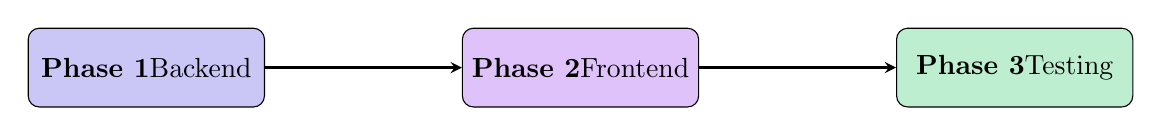
\begin{tikzpicture}[node distance=1.5cm]
  \tikzstyle{phase} = [rectangle, rounded corners, minimum width=3cm, minimum height=1cm, text centered, draw=black, fill=blue!20]
  \tikzstyle{arrow} = [thick,->,>=stealth]

  \node (phase1) [phase, fill=primaryblue!30] {\textbf{Phase 1}\\ Backend};
  \node (phase2) [phase, fill=secondarypurple!30, right=of phase1, xshift=1cm] {\textbf{Phase 2}\\ Frontend};
  \node (phase3) [phase, fill=successgreen!30, right=of phase2, xshift=1cm] {\textbf{Phase 3}\\ Testing};

  \draw [arrow] (phase1) -- (phase2);
  \draw [arrow] (phase2) -- (phase3);
\end{tikzpicture}
\caption{Implementation timeline}
\end{figure}

\begin{itemize}
  \item \textbf{Phase 1:} Build the backend (database, AI integration, intelligence gathering)
  \item \textbf{Phase 2:} Build the frontend (chat interface, SwitchIT integration)
  \item \textbf{Phase 3:} Final testing and beta launch preparation
  \item \textbf{Post-Launch:} Beta testing with initial users, gather feedback, iterate
\end{itemize}

%===============================================
\section{Conclusion}
%===============================================

\subsection{What We're Building}

We're creating an intelligent career companion that:
\begin{itemize}
  \item Provides personalized guidance based on your unique journey
  \item Learns from thousands of users to give market-validated insights
  \item Remembers your conversations and context over time
  \item Costs 95\% less than typical AI systems (\$20-40/month for 1,000 users)
  \item Respects your privacy with clear controls and transparency
\end{itemize}

\subsection{Why It Matters}

This transforms SwitchIT from a static professional profile platform into a \textbf{dynamic career growth platform}. Users don't just list their experience—they actively develop it with AI-powered guidance.

\subsection{Next Steps}

\begin{enumerate}
  \item \textbf{Immediate:} Review this plan and provide feedback
  \item \textbf{Week 1:} Start backend developmen
  \item \textbf{Week 3:} Begin frontend developmen
  \item \textbf{Week 4:} Beta launch with select users
  \item \textbf{Month 2:} Iterate based on feedback, expand to more users
  \item \textbf{Month 3:} Full public launch
\end{enumerate}

\begin{keypoint}
\textbf{Success means:} Users feel like they have a supportive career mentor in their pocket, always available to help them navigate their professional journey—and SwitchIT becomes the platform that truly helps people grow, not just connect.
\end{keypoint}

\end{document}
